\newpage
\section{Anhang}

\subsection{Versuchsaufbauten}
\begin{figure}[H]
    \centering
    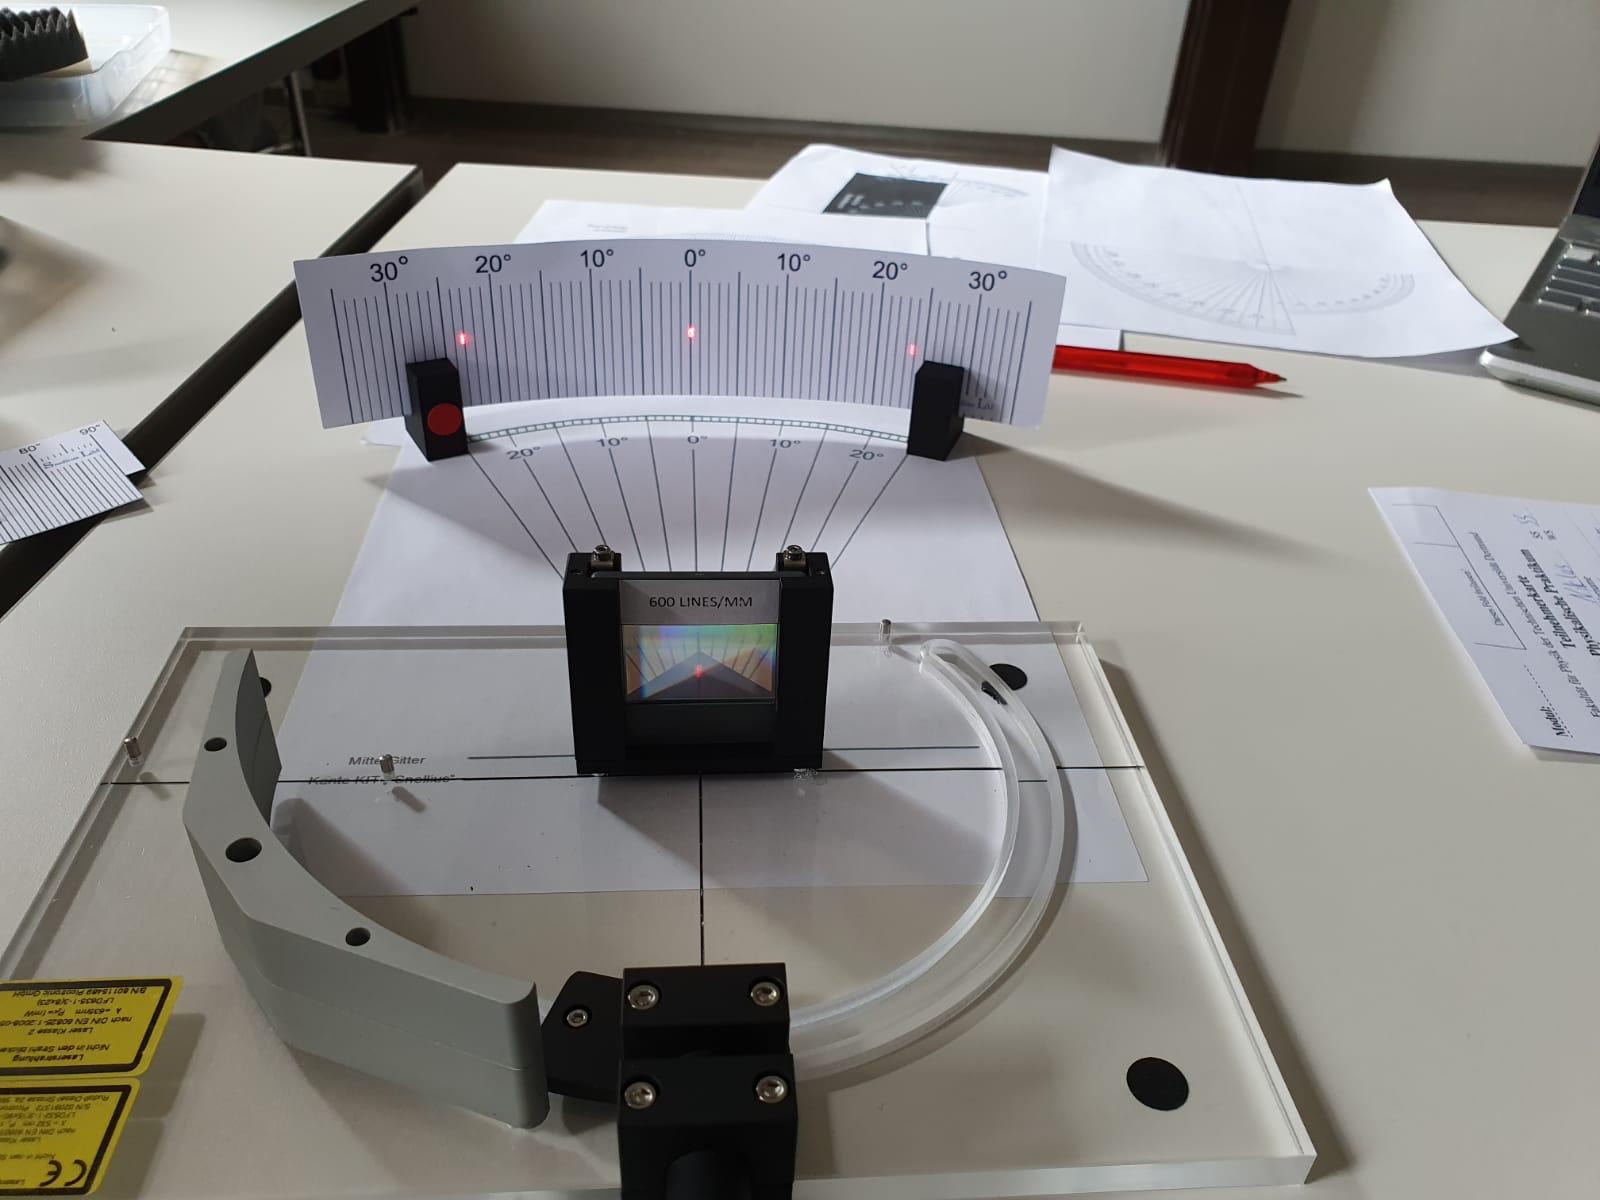
\includegraphics[width=0.63\textwidth]{latex/images/gitter.jpeg}
    \caption{Ein Foto des Aufbaus um Interferenz zu untersuchen.}
    \label{img:aufbaugitter}
\end{figure}

\begin{figure}[H]
    \centering
    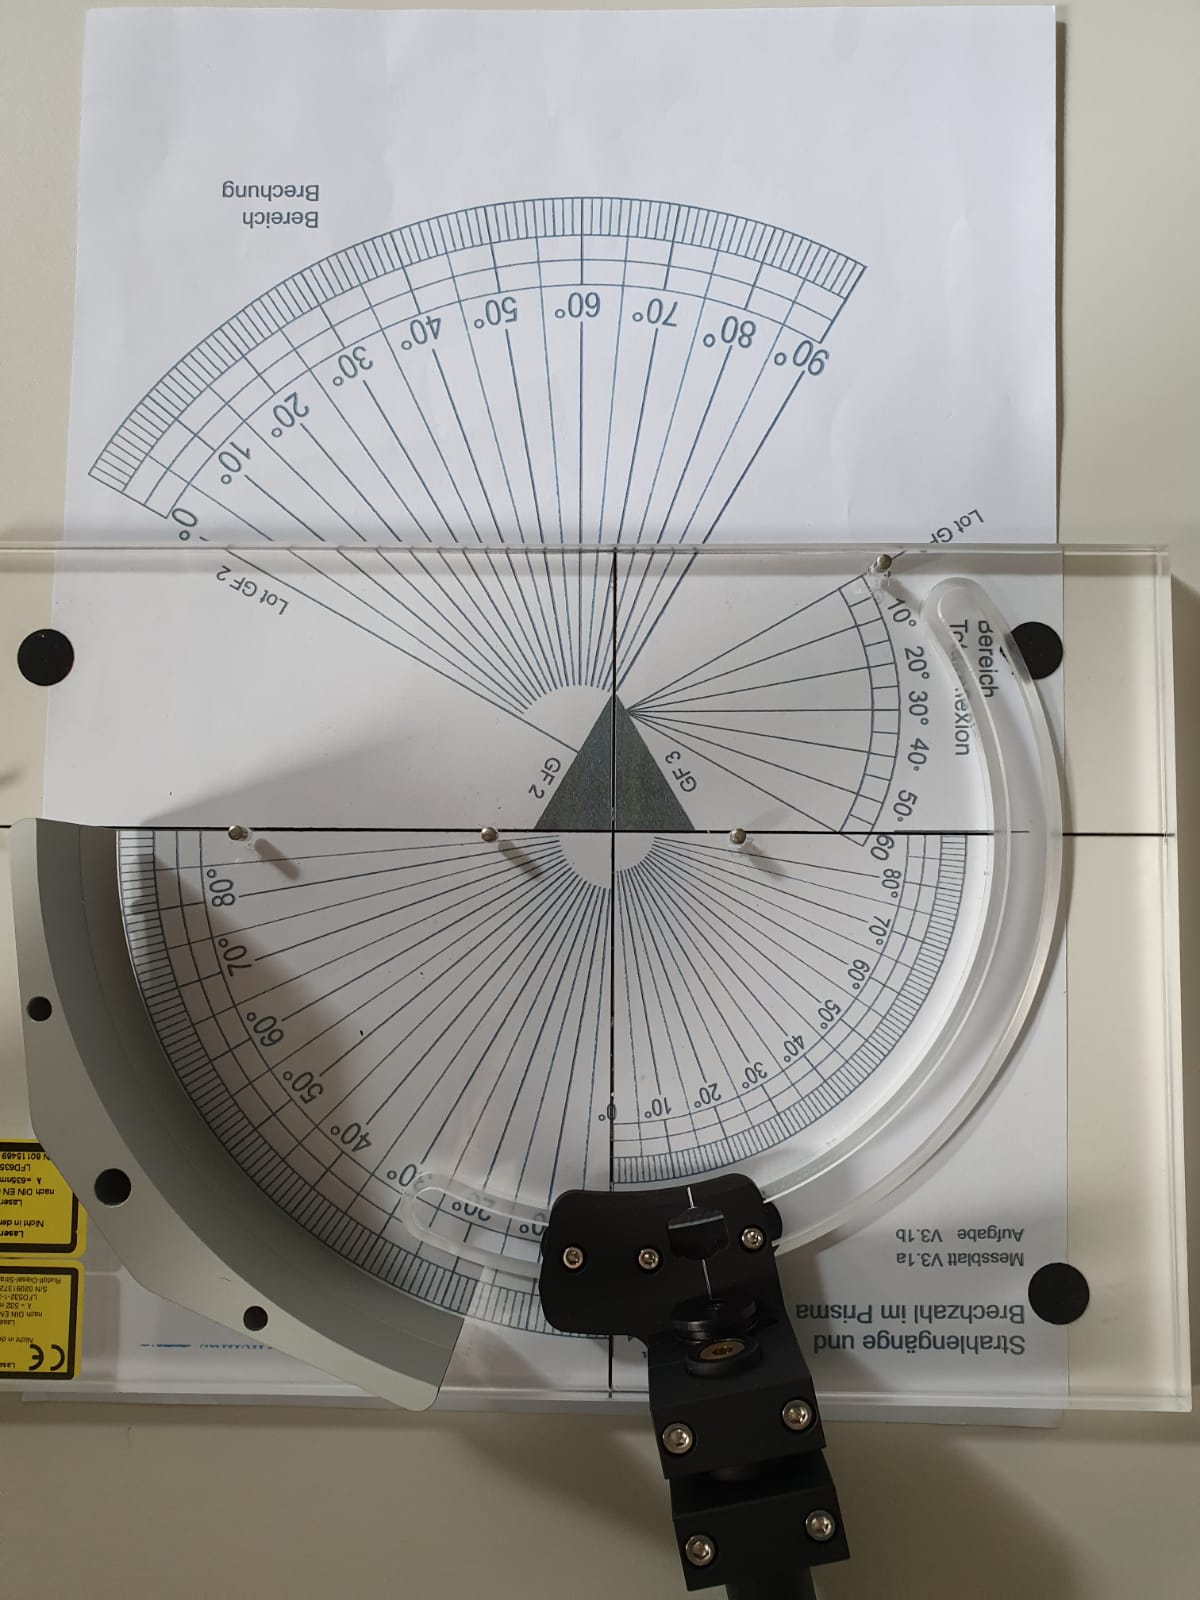
\includegraphics[width=0.63\textwidth]{latex/images/prisma.jpeg}
    \caption{Ein Foto des Aufbaus um die Brechung des Lichts an einem Prisma zu untersuchen.}
    \label{img:aufbauprisma}
\end{figure}


\subsection{Daten}
\begin{figure}[H]
    \centering
    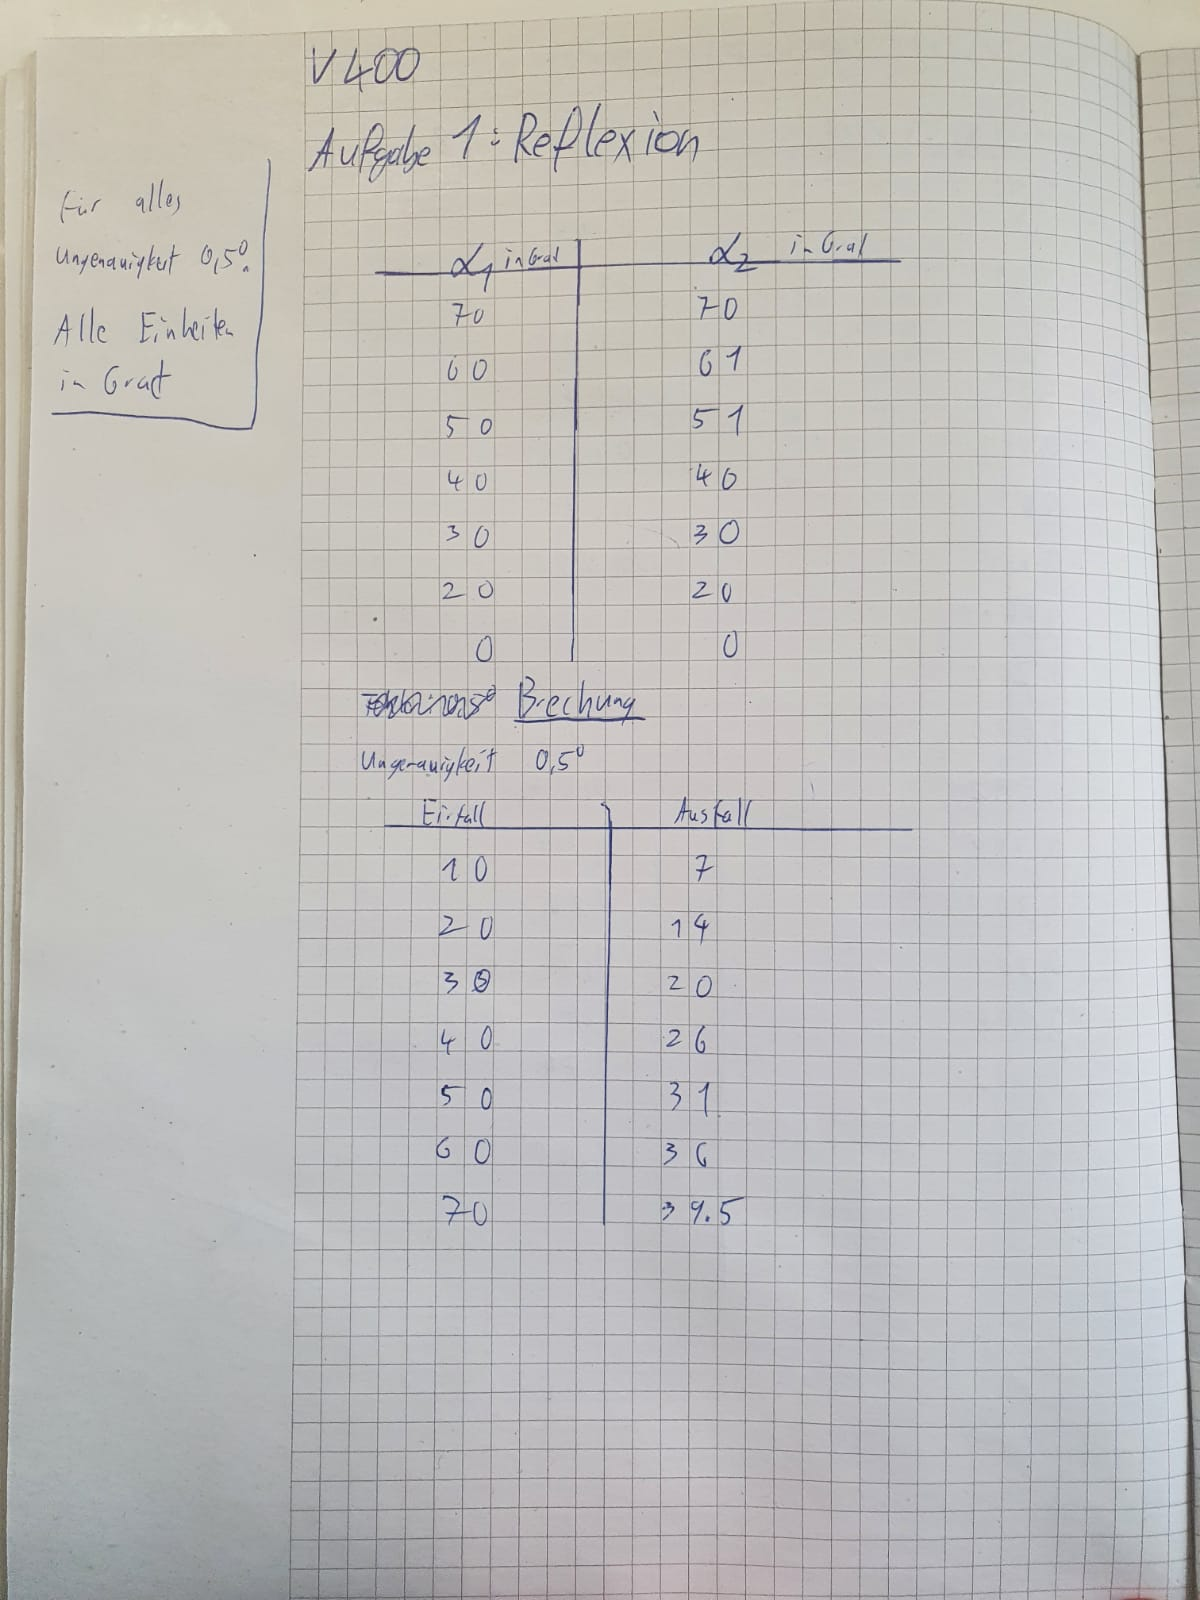
\includegraphics[width=0.63\textwidth]{latex/images/werte1.jpeg}
    \caption{Ein Foto der Messdaten.}
    \label{img:Daten1}
\end{figure}
\begin{figure}[H]
    \centering
    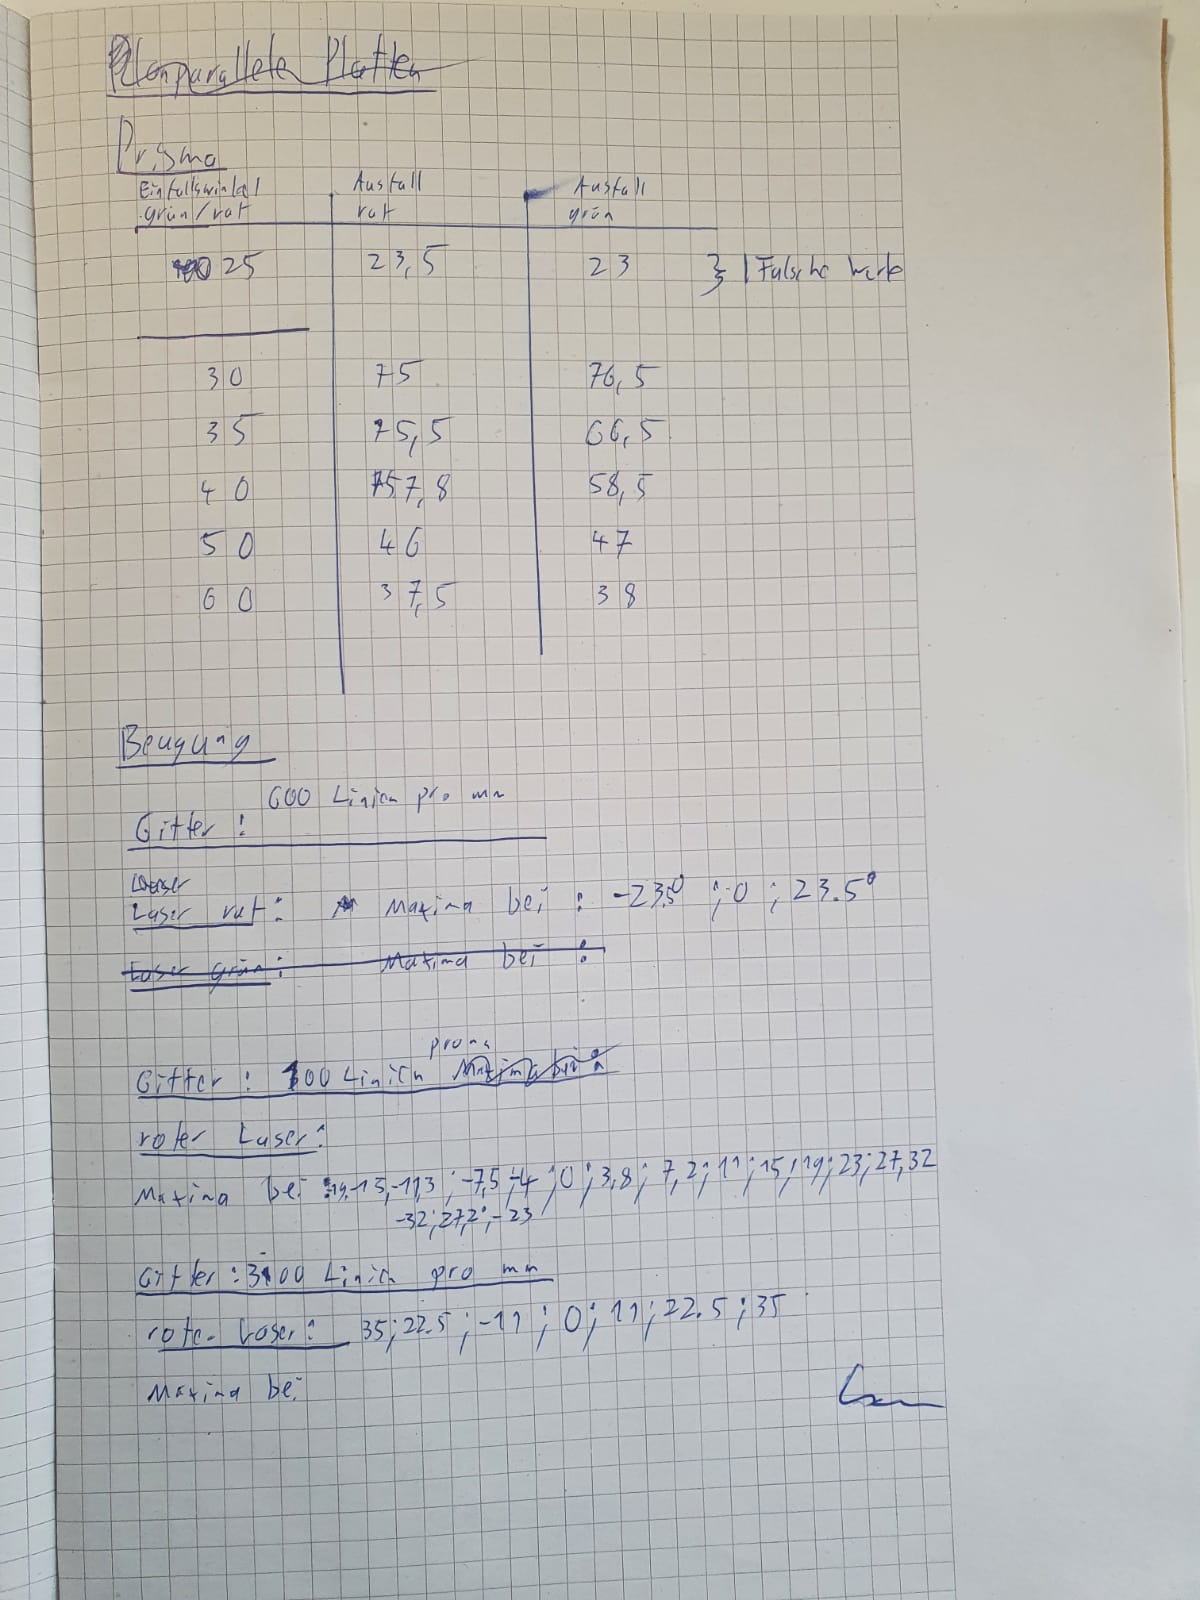
\includegraphics[width=0.63\textwidth]{latex/images/werte2.jpeg}
    \caption{Ein Foto der Messdaten.}
    \label{img:Daten2}
\end{figure}


\begin{table}[H]
    \centering
    \begin{tabular}{S [table-format=2.2] S [table-format=3.2]}
        \toprule
        {$U \mathbin{\scalebox{1.5} / }\si{\volt}$} & {$I \mathbin{\scalebox{1.5} / }\si{\ampere}$}\\
        \midrule
         19.02 & 0.00\\
         15.00 & 0.00\\
         10.00 & 0.00\\
         5.00  & 0.00\\
         2.51  & 0.00\\
         0.49  & 0.02\\
         0.25  & 0.82\\
         0.15  & 1.90\\
         0.05  & 4.10\\
         0.01  & 5.20\\
        -0.05  & 6.40\\
        -0.15  & 9.50\\
        -0.25  & 12.00\\
        -0.35  & 14.50\\
        -0.50  & 16.30\\
        -0.75  & 24.00\\
        -1.00  & 29.00\\
        -1.52  & 36.00\\
        -2.50  & 51.00\\
        -5.01  & 74.00\\
        -10.01 & 94.00\\
        -15.02 & 102.00\\
        -19.12 & 105.00\\
        \bottomrule
    \end{tabular}
\caption{Die Messwerte der Messreihe vom gelben Licht.}
\label{tab:gelb}
\end{table}
